\subsection{NV Center Platform}
\label{qnodeos:sec:qdevice-nv}

The \ac{QDevice} employed for the benchmark experiments is constituted by an \ac{NV} center processor. We use the \ac{NV} center in its negatively charged state (called \ac{NV}$^-$) for quantum information processing. \ac{NV}$^-$ is a spin-1 system, whose ground states are non-degenerate in the presence of an external magnetic field, see \cref{fig:nv_levels}~\cite{doherty_2013}. We employ the $m_s=0$ as our $\ket{0}$ state for the qubit, while for the $\ket{1}$ we can choose one of $m_s=\pm 1$. Details on how the choice is made will follow in the next section. The \ac{NV} can be optically excited resonantly (637\,nm) and off-resonantly (typically 532\,nm), and it emits in 3\% of the cases single photons (\ac{ZPL} photons), while the remaining part is constituted by the emission of a photon and a phonon (\ac{PSB}). The optical transitions are spin-selective, as shown in~\cref{fig:nv_levels}. In the presence of lateral strain and external DC field (Stark effect), the excited states of the \ac{NV} split apart, maintaining their spin-selective properties. In this work, we use a natural lateral strain between 2\,GHz and 5\,GHz. The cycling transition denoted as \ac{RO} in \cref{fig:nv_levels} is used to emit single photons (\ac{ZPL}) for entanglement generation and to read out the state of the qubit (fluorescence in the \ac{PSB}). From the excited states, the \ac{NV} can also decay through metastable states (not shown in \cref{fig:nv_levels}). The preferable decay from such metastable states is the $m_s=0$ state. In this way, it is possible to optically initialize the qubit state to $\ket{0}$ (dashed line in~\cref{fig:nv_levels}), with fidelity above 99\%, when on-resonantly exciting the \ac{SP} transition and averaging for long enough to ensure a spin-flip. In our experiments, we apply a laser field on resonance with the \ac{SP} transition at 500\,$n$W for 1.5\,$\mu$s for fast initialization during entanglement attempts, whereas a slow initialization (10\,$n$W for 100\,$\mu$s) is used for single-qubit gates experiments (like local tomography). On the other hand, while exciting the \ac{RO} transition, decays to $m_s=\pm 1$ are also possible, but they present longer cyclicity. This feature is relevant for the optical read-out of the qubit state, which can be done in a single shot and is discussed in the following sections.

\begin{figure}
    \centering
    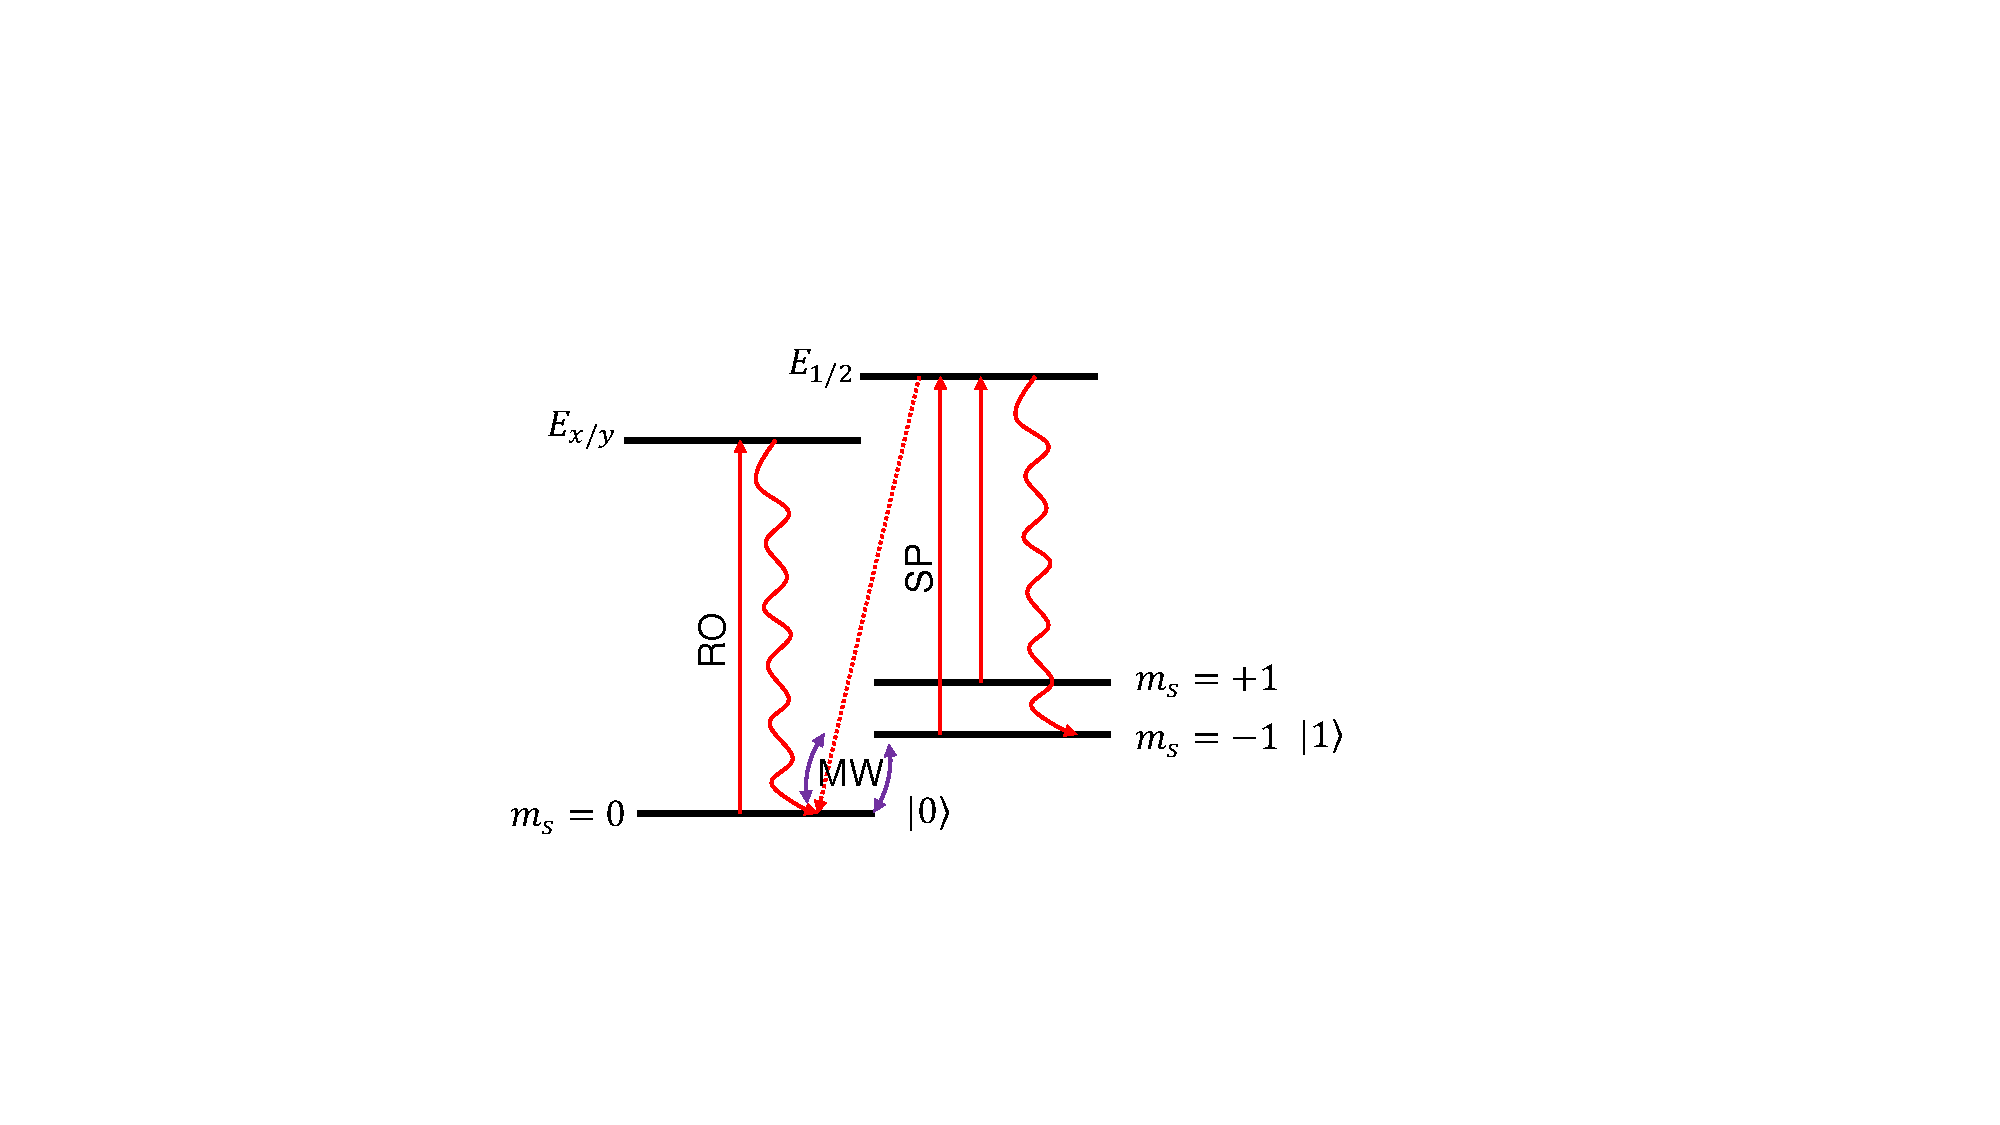
\includegraphics[width=0.8\linewidth]{figures/qnodeos/supplementary/levels_NV.pdf}
    \caption{Energy structure of \ac{NV}$^-$ at 4\,K. The ground state of the \ac{NV} splits into three distinct levels (Zeeman splitting). The optical transitions are spin-selective. The excited states are represented as one, but they are non-degenerate when lateral strain is applied. We denote as \acf{RO} the transition $\ket{0}\rightarrow E_{x/y}$ and as \acf{SP} the transition $\ket{1}\rightarrow E_{1/2}$. The wiggly lines represent the photoluminescence when such transitions are excited, whereas the dashed lines represent the decay via metastable states that is used for initialization of the qubit state into $\ket{0}$. \acf{MW} pulses enables the transfer of population between the two states of the qubit, allowing for quantum information processing.}
    \label{fig:nv_levels}
\end{figure}

In our demonstration, the server has an external magnetic field of $B_z=189$\,mT aligned along the symmetry axis $z$ of the \ac{NV}, while the client experiences $B_z=23$\,mT. The magnetic field is applied via permanent magnets placed both inside and outside the high-vacuum chamber of our closed-cycle cryostats. Fluctuations of the magnetic field are observed on the order of nT on a timescale of hours, therefore they do not constitute a limitation for our demonstration. We also measured a perpendicular component of the permanent magnetic field for both setups of $\sim$1\,mT. Such misalignment becomes crucial for the coherence time of the electron spin qubit, as in the interaction with the surrounding nitrogen nuclear spins, the off-axis hyperfine interaction terms become non-negligible and the decoupling of the electron spin is harder~\cite{doherty_2013}. Notably, the server node is in the regime of ``high magnetic field''. In the level structure depicted in \cref{fig:nv_levels}, this means that the $m_s=-1$ ground state crossed the $m_s=0$ state (at $\sim$\,100mT), and the optical transitions for the \ac{SP} are well separated, such that a double laser field with proper detuning is necessary to correctly address both of them.

\subsubsection{Single Node Operations}

In this section, details on how to operate a single node for quantum information processing are given. The physical setup is the one employed for the demonstration in Ref.~\cite{pompili_2022_experimental}.

\paragraph{Charge-resonance check}

To use the \ac{NV} as a processing node, it is necessary to guarantee that it is in the correct charge state and the laser fields are on resonance with the transitions. Before executing any instructions coming from the \ac{QNPU}, both nodes go through the so-called \ac{CR} check. We apply resonant fields for 100\,$\mu$s on both the \ac{RO} (1\,$n$W) and \ac{SP} (10\,$n$W) transitions and we monitor the fluorescence. If the number of photons exceeds the threshold (25 for the client and 60 for the server for our experiments), the node is considered ready to accept instructions from the \ac{QNPU} and can proceed with synchronization with the other node (for multinode instructions). The threshold is set considering the brightness of each \ac{NV}. The success is considered valid for 100\,$m$s. After this time, if no instructions arrive, the \ac{CR} check is repeated. In case the number of photons is below the threshold, we distinguish two cases: (1) the counts are between the success threshold and a second threshold called Repump: we repeat the \ac{CR} check and tune the frequency of the red lasers, as they might not address the transitions correctly; (2) the number of counts is below the Repump threshold (set at 15 for the client and 25 for the server): this means that the \ac{NV} might be in the dark charge state (\ac{NV}$^{0}$) due to ionization. To restore the charge state, in the next round of \ac{CR} check we first illuminate with off-resonant green laser (20\,$\mu$W for 50\,$\mu$s), or, for the client node only, with yellow light (575\,nm, 35\,$n$W for 300\,$\mu$s) on resonance with the \ac{ZPL} transition of \ac{NV}$^{0}$~\cite{baier_2020}. This is necessary because we additionally apply an external DC field to the \ac{NV} on the client node. We, indeed, exploit the Stark effect to tune the \ac{RO} transition to be the same as the server's one \cite{basssett_2011}. In this way, we can ensure photon indistinguishability in frequency that is crucial for entanglement generation. The typical DC field used for this work is $\sim$2V, modulated via an error signal that is computed on the \ac{CR} check counts, acting as a \ac{PID} loop.

The \ac{CR} check is repeated after an experiment iteration. This round is utilized to validate the experiment and post-select the results based on success or failure of this procedure, as discussed in \cref{qnodeos:sec:methods}.

\paragraph{Single qubit gates}

To manipulate the state of the electron spin qubit, microwave pulses are on resonance with the transition $\ket{0}\rightarrow\ket{1}$ are employed. For the server node, the $m_s=-1$ state is used as $\ket{1}$ and the resonance frequency is 2.4\,GHz. The client node utilizes the $m_s=+1$, with a resonance frequency of 3.5\,GHz. The choice of the $\ket{1}$ is made based on the gate fidelity.

We use skewed-Hermite \acf{MW} pulses~\cite{warren_1984,vandersypen_2005} with high Rabi frequency ($\sim$10\,MHz), which generates an alternating magnetic field capable of manipulating the state of the qubit. The characterizing values for the two nodes are reported in Table \ref{tab:mw_pulse}. The measured infidelity on a single \ac{MW} pulse is below 1\%. Instructed by the \ac{QNPU}, we performed local quantum tomography on both the server and the client, showing high fidelity. One example is reported in \cref{fig:tomography-no-multitasking}.

\begin{table}[]
    \centering
    \begin{tabular}{|r|c|c|}
    \hline
 &Client & Server\\
\hline
        Duration $\pi$ rotation & 200\,$n$s & 190\,$n$s\\
        Amplitude $\pi$ rotation & 0.78 & 0.89\\
        Skewness $\pi$ rotation & -1.5e$^{-9}$ & -3.5e$^{-9}$\\
        Duration $\pi/2$ rotation & 150\,$n$s&  100\,$n$s\\
        Amplitude $\pi/2$ rotation & 0.38 & 0.56\\
        Skewness $\pi/2$ rotation & -1.2e$^{-8}$& -7.1e$^{-9}$ \\
        Power & 42\,W & 42\,W\\
        \hline
    \end{tabular}
    \caption{Characterizing values for the \ac{MW} pulses. Other rotation angles have the same duration and skewness as the $\pi$ pulse, and the amplitudes scale accordingly. The rotation axes are obtained by changing the phase of the pulse. With the current setup configuration, only rotations along $\hat{x}$ and $\hat{y}$ axes are feasible, so $\hat{z}$ rotations are compiled as combinations of gates along $\hat{x}$ and $\hat{y}$.}
    \label{tab:mw_pulse}
\end{table}

\paragraph{Dynamical decoupling}

Once \ac{MW} pulses are set up with high fidelity, it is possible to implement \ac{DD} sequences that increase the coherence time of the electron spin qubit. \ac{DD} sequences are especially crucial in our experiments when the latency of the \ac{QNPU} is long (milliseconds timescale), like in the \ac{DQC} demonstration. The characterizing parameter for a \ac{DD} sequence is the time delay between the $X$ and $Y$ pulses. To optimize it, we swept the interpulse delay, at the sample precision of our Arbitrary Waveform Generator (0.42\,$n$s, Zurich Instruments HDAWG), while playing the effective single-qubit computation of the \ac{DQC} protocol instructed by the \ac{QNPU}, as explained in \cref{qnodeos:sec:methods}, on both the client and the server. In doing so, we added an extra waiting time of 5\,$m$s between the initialization of the qubit into the superposition state and the subsequent gates to mimic the real-case scenario of the \ac{DQC}. In this way, we are able to set the optimal interpulse delay, obtaining a single-qubit fidelity of 0.96(2) for the server and 0.88(2) for the client.

\paragraph{Single-shot readout}

When a measurement instruction arrives from the \ac{QNPU}, this is translated by the physical layer as a Single-Shot Readout measurement. To assign a state to the qubit, we can use the \ac{RO} optical transition. The \ac{RO} laser field is on for $\sim$10\,$\mu$s at 1\,$n$W. This will produce fluorescence only if the \ac{NV} is in the $\ket{0}$ state. If no photons are detected while the laser is on, the outcome is assigned to the $\ket{1}$ state. The fidelity of the measurement process is defined as $F=1/2(F_{0|0}+F_{1|1})$, where $F_{0|0}$ ($F_{1|1}$) represents the fidelity of measuring $\ket{0}$ ($\ket{1}$) when the qubit is prepared in $\ket{0}$ ($\ket{1}$). For our experiments, we obtain 0.841(4) and 0.997(1) respectively for the client, and 0.912(3) and 0.995(1) for the server, achieving above 0.90 of process fidelity.

\subsubsection{Entanglement generation}
\label{qnodeos:sec:NVentanglement}

The entanglement request from the \ac{QNPU} is translated into executing a single-photon protocol. The communication qubit on each node is initialized in the state $\sqrt{\eta} \ket{0} + \sqrt{1-\eta} \ket{1}$, where $\eta$ represents the bright state population. For maximum state fidelity, the condition $\eta_C p_C \approx \eta_S p_S$ applies, where $\eta_{C(S)}$ is the bright state population of the client (server) and $p_{C(S)}$ is the photon detection probability of the client (server). In this work, $\eta_{C}=0.07$ and $\eta_S = \eta_C \frac{p_C}{p_S} = 0.04$. The choice of $\eta_C$ is a trade-off between entangled state fidelity and entanglement generation rate. The produced entangled state is (non-deterministically) one of two Bell states $\ket{\Psi^\pm} = \frac{1}{\sqrt{2}}(\ket{01} \pm e^{i\Delta\theta}\ket{10})$, based on which detector clicked at the heralding station. The phase $\Delta\theta$ is actively stabilized~\cite{pompili_2021_multinode} before the execution of the entanglement request, via a combination of homodyne interference, for the global phase of the network, and a heterodyne interference, to stabilize the local phase at each node. Pauli-correction gates, based on the state prepared, are issued from the server \ac{QNPU} to its \ac{QDevice} to obtain $\ket{\Phi^+}$: an $X_{\pi}$ gate if the generated Bell-state is $\ket{\Psi^+}$ and an $X_{\pi}$ gate followed by a $Z_{\pi}$ gate (decomposed into X and Y gates) for $\ket{\Psi^-}$. As preparation for the experiment, we verified the entanglement generation, instructed by the \acp{QNPU} and using the same method as in Ref.~\cite{pompili_2022_experimental}, achieving a fidelity of $0.72(\pm 0.02)$ for the $\ket{\Phi^+}$ state. The Bell corrections done through the server \ac{QNPU} take up to 0.16 ms for $\ket{\Psi^+}$ and up to 0.49\,ms for $\ket{\Psi^-}$. On the other hand, generating entanglement without the \ac{QNPU} and with no Pauli correction, we achieve an average fidelity of 0.74($\pm$0.03), with $\eta_{C}=0.1$ and $\eta_S=0.06$. The choice of different $\eta$ values is due, in the first place, to speed up the rate of such a measurement. It shows, however, better performance with respect to the instructed version, which is due to the fact that the Pauli-correction instruction comes with a latency.